
\section{Deriving and Analyzing a Corresponding Deferrable Task Set}
\label{sec:convert}

To apply an analysis of the period enforcer based on Theorem 5 in~\cite{Raj:suspension1991}, we need to convert a given set of multi-segment self-suspending tasks into a corresponding set of single-segment deferrable tasks. This raises two questions: first, how can we efficiently derive the corresponding set of single-segment deferrable tasks? And second, how should we perform the schedulability test on the corresponding single-segment deferrable tasks correctly? We will discuss the difficulty of deriving a suitable corresponding task set in Section~\ref{sec:transformation-exponential} and the potential for pessimism in any schedulability test based on the set of single-segment deferrable tasks  in Section~\ref{sec:schedulability-test-deferrable}.

\subsection{Task Set Transformation}
\label{sec:transformation-exponential}

The needed transformation from a multi-segmented self-suspending task to a corresponding set of single-segment deferrable tasks was not discussed in \cite{Raj:suspension1991}. However, in our opinion, performing such a transformation without introducing additional pessimism is not easy in the general case, nor is it obvious how to do so.

We demonstrate the inherent difficulty of the problem by focusing on a special case to which we can apply a recent result of Nelissen et al. \cite{ecrts15nelissen}, which allows analyzing the exact worst-case response time of multi-segmented self-suspending sporadic tasks, albeit with exponential time complexity. 
Nelissen et al.'s worst-case response time analysis~\cite{ecrts15nelissen} is exact under the following conditions:\footnote{We refer to the characteristics of the worst-case release pattern provided in Lemma 2 in \cite{ecrts15nelissen}. The exact worst-case response time can be obtained by exploring all  release patterns that satisfy these conditions.} 
\begin{enumerate}
	\item the task set contains only one self-suspending task, 
	\item the self-suspending task is the lowest-priority task, 
	\item the scheduling policy is preemptive fixed-priority scheduling, and 
	\item all tasks have constrained deadlines.	
\end{enumerate}


Suppose that the system has $k-1$ regular sporadic tasks and only one segmented self-suspending task $\tau_k$, and that all tasks have implicit deadlines ($T_i = D_i$ for all $\tau_i$). Further suppose that task $\tau_k$ has $m_k$ segments with $m_k \geq 3$.  To  convert a computation segment into a single-segment deferrable task, we need to derive the segment's \emph{latest-possible arrival time}, relative to the release of the job. Formally,  for the $j^{\mathrm{th}}$ computation segment of task $\tau_k$, we let $\rho_k^j$ denote its latest-possible arrival time, with the interpretation that, if a job of task $\tau_k$ arrives at time $t$, then  it is guaranteed that the $j^{\mathrm{th}}$ computation segment of this job will arrive no later than at time $t+\rho_k^j$.

How can we compute $\rho_k^j$? Suppose that the worst-case response time of the $j^{\mathrm{th}}$ computation segment of task $\tau_k$ is $W_k^j$, and recall that $S_k^{j}$ denotes the maximum self-suspension length before the $j^{\mathrm{th}}$ computation segment of $\tau_k$. Then $\rho_k^j$ can be expressed in terms of $W_k^{j-1}$:
$$
	\rho_k^j = W_k^{j-1}+S_k^{j-1},
$$
where $W_k^0$.  Therefore, if we can derive the exact $W_k^j$ for $j=1,2,\ldots,m_k-1$ for task $\tau_k$, we can easily compute $\rho_k^j$  for $j=1,2,\ldots,m_k$. And conversely, if we can somehow compute $\rho_k^j$  for $j=2,\ldots,m_k$, we  can trivially infer $W_k^j$ for $j=1,2,\ldots,m_k-1$.
Based on these considerations, it appears that the transformation problem is  --- at least in the considered special case --- equivalent to worst-case response time analysis of multi-segmented self-suspending task systems. 

However, deriving an exact bound $W_k^j$ for $j=1,2,\ldots,m_k-1$ for task $\tau_k$ is not easy at all: 
even for the above ``simple'' case, Nelissen et al.'s solution~\cite{ecrts15nelissen} for calculating the exact worst-case response time requires exponential time complexity if $j \geq 2$. Furthermore, Nelissen et al. \cite{ecrts15nelissen} identified several misconceptions in prior analyses, and after correcting those misconceptions, observed that deriving the worst-case response time of a computation segment in pseudo-polynomial time seems to be a very challenging problem indeed.\footnote{In fact, in ongoing work, this problem has recently been shown to be coNP-hard in the strong sense~\cite{Chen2016b}.}

In the context of the period enforcer, we consequently observe that the only existing solution for deriving the \emph{precise} bound $W_k^{j}$ (and hence $\rho_k^j$), due to Nelissen et al.\ \cite{ecrts15nelissen},  has exponential time complexity (even for the considered special case of a single self-suspending task). If over-approximations can be tolerated, finding a safe upper bound on $W_k^j$ for $j=1,2,\ldots,m_k-1$ can be done in pseudo-polynomial time \cite{PH:rtss98,Huang:multiseg}, albeit at a loss of accuracy and hence generality. 


\subsection{Schedulability Test for A Corresponding Deferrable Task Set}
\label{sec:schedulability-test-deferrable}

Suppose that the corresponding deferrable task set can be derived precisely by ignoring the complexity issues raised in Section~\ref{sec:transformation-exponential}. The next question is whether there is any information loss, with respect to the schedulability test, by inspecting only the corresponding deferrable task set. We will demonstrate an example to explain the information loss.

Consider a task system consisting of $2$ tasks. Let $\tau_1$ denote a sporadic task without self-suspensions, in which $C_1 = 2$ and $T_1=D_1=10$. Let $\tau_2$ denote a self-suspending task consisting of three computation segments with parameters  $C_2^1 = 1$,  $S_2^1 = 6$, $C_2^2=1$, $S_2^2=8$, $C_2^3=1$, and $ T_2=D_2=21$. That is, this task set is pretty similar to the task set used in Section~\ref{sec:unschedulable}. One additional computation
segment is created to illustrate the potential concerns. This task set is schedulable by fixed-priority preemptive scheduling without any enforcement since the worst-case response time of the second computation segment is $10$ and the third computation segment will suffer from the interference by at most one job from task $\tau_1$. Moreover, by using the analysis in Section~\ref{sec:transformation-exponential}, we can conclude that
\begin{equation*}
  \rho_2^1 = 0, \rho_2^2 = 9, \rho_2^3 = 18.
\end{equation*}
Therefore, in the corresponding deferrable task set, there are $2$ sporadic tasks $\tau_1$ and $\tau_2^1$ (with execution time $1$ and period $21$), and two deferrable tasks $\tau_2^2$ (with deferrable length $9$, period $21$, and execution time $1$) and $\tau_2^3$ (with deferrable length $18$, period $21$, and execution time $1$).  

Suppose that we are interested to analyze the worst-case response time of the deferrable task $\tau_2^3$ (in the corresponding deferrable task set) under fixed-priority scheduling. The question is \emph{whether we should ignore or should include the interference due to $\tau_2^1$ and $\tau_2^2$}.
Since the computation segments that are used to create $\tau_2^1, \tau_2^2$, and $\tau_2^3$ do not have any overlap in their available time to be executed, it may be seemingly correct at beginning that we do not have to consider the interference from $\tau_2^1$ and $\tau_2^2$ when analyzing the response time of the deferrable task $\tau_2^3$. However, this statement is in fact incorrect.


If we do not consider the interference from $\tau_2^1$ and $\tau_2^2$, we can conclude that the worst-case response time of $\tau_2^3$ is  $18+C_1+C_2^3=21$.
Let us consider this task set under the control of the period enforcer algorithm, as defined in Section \ref{sec:pe}.
Figure \ref{fig:example-deferrable-incompatible} shows the resulting schedule for a periodic release pattern. This changes the schedule of the second job of task $\tau_2$. 
The second job of task $\tau_2$ (which is released at time $21$) is affected by period enforcement. The first segment of the second job arrives at time $a^1_{2,2} = 21$, is interfered for one time unit, and suspends at time $23$. The  second segment of the second job hence resumes only at time $a^2_{2,2} = 29$. Thus, we have
\begin{align*}
	ET_{2,2}^1 & = \max\left(0 + 21,\ \mathit{busy}(\tau_2, 21)\right) = 21  \text{ and }
\\
	ET_{2,2}^2 & = \max\left(9 + 21,\ \mathit{busy}(\tau_2, 29\right) ) = 30.
\end{align*}
According to the rules of the period enforcer algorithm, the processor therefore remains idle at time $29$ because the segment is not eligible to execute until time $ET_{2,2}^2 = 30$. However, at time $30$, the fourth job of $\tau_1$ is released. As a result, the second job of $\tau_2$ suffers from additional interference and misses its deadline at time $42$.

If we further allow task $\tau_1$ to be released sporadically, the fifth job of task $\tau_1$ can be released at time $41$ instead of time $40$ in Figure~\ref{fig:example-deferrable-incompatible}. For such a case, the response time of the second job of task $\tau_2$ is $23$. This means that the worst-case response time of the deferrable task$\tau_2^3$ must be at least $23$, which equals to $18+C_1 + C_2^1+C_2^2+C_2^3$.

Therefore, for this specific example, we know that the schedulability test for the  corresponding deferrable task set has also to be pessimistic enough to consider the interferences from all the computation segments created from the same self-suspending sporadic task.

\begin{figure}[t]
  \centering  
  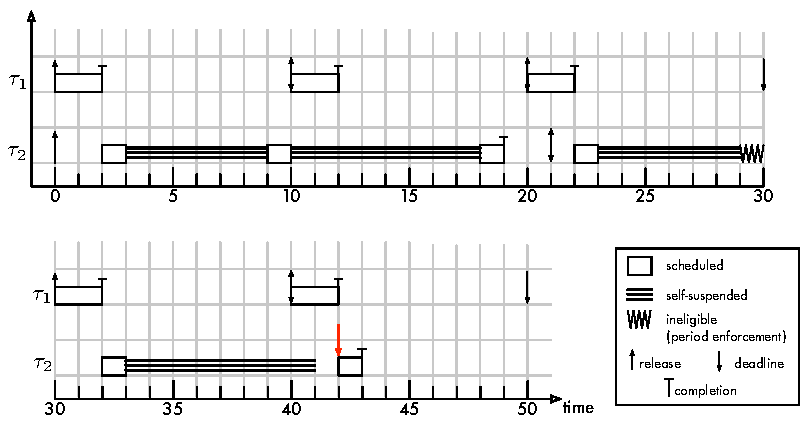
\includegraphics[scale=1]{../figures/deferrable-incompatible/deferrable-incompatible.pdf}
  \caption{An example for explaining why it is not safe to ignore the interference from the other computation segments in the same task.}
  \label{fig:example-deferrable-incompatible}
\end{figure}

\subsection{Discussions}
\label{sec:discussions-deferrable}

The transformation from a segmented self-suspending task set to a corresponding deferrable task set and the corresponding schedulability test were not discussed in \cite{Raj:suspension1991}. With the above discussions in Section~\ref{sec:transformation-exponential} and Section~\ref{sec:schedulability-test-deferrable}, we find that the transformation is in fact non-trivial and the schedulability test of the corresponding deferrable task set has also to be pessimistic. As shown in Section~\ref{sec:schedulability-test-deferrable}, even if we derive the precise deferrable time (release jitter) information, we may still have to account for the computation segments that have no \emph{direct} interference with a computation segment that is under analysis (e.g., the third computation segment of task $\tau_2$ in Section~\ref{sec:schedulability-test-deferrable}).

Fundamentally, the design of the period enforcer algorithm relies on the schedulability of a deferrable task set. However, as we demonstrated here, there is a gap between the segmented self-suspending task set and the corresponding deferrable task set in the transformation and also in the schedulability test analysis. The authors in this paper do not find any simple way to provide a schedulability test without any information loss.

%%% Local Variables:
%%% mode: latex
%%% TeX-master: "LITES/LITES-Paper.tex"
%%% End:
